% Options for packages loaded elsewhere
\PassOptionsToPackage{unicode}{hyperref}
\PassOptionsToPackage{hyphens}{url}
%
\documentclass[
  english,
  man,floatsintext]{apa6}
\usepackage{amsmath,amssymb}
\usepackage{lmodern}
\usepackage{iftex}
\ifPDFTeX
  \usepackage[T1]{fontenc}
  \usepackage[utf8]{inputenc}
  \usepackage{textcomp} % provide euro and other symbols
\else % if luatex or xetex
  \usepackage{unicode-math}
  \defaultfontfeatures{Scale=MatchLowercase}
  \defaultfontfeatures[\rmfamily]{Ligatures=TeX,Scale=1}
\fi
% Use upquote if available, for straight quotes in verbatim environments
\IfFileExists{upquote.sty}{\usepackage{upquote}}{}
\IfFileExists{microtype.sty}{% use microtype if available
  \usepackage[]{microtype}
  \UseMicrotypeSet[protrusion]{basicmath} % disable protrusion for tt fonts
}{}
\makeatletter
\@ifundefined{KOMAClassName}{% if non-KOMA class
  \IfFileExists{parskip.sty}{%
    \usepackage{parskip}
  }{% else
    \setlength{\parindent}{0pt}
    \setlength{\parskip}{6pt plus 2pt minus 1pt}}
}{% if KOMA class
  \KOMAoptions{parskip=half}}
\makeatother
\usepackage{xcolor}
\IfFileExists{xurl.sty}{\usepackage{xurl}}{} % add URL line breaks if available
\IfFileExists{bookmark.sty}{\usepackage{bookmark}}{\usepackage{hyperref}}
\hypersetup{
  pdftitle={It's Time To Abandon the Cross-Lagged Panel Model},
  pdfauthor={Richard E. Lucas1},
  pdflang={en-EN},
  pdfkeywords={cross-lagged panel model, longitudinal, structural equation modeling},
  hidelinks,
  pdfcreator={LaTeX via pandoc}}
\urlstyle{same} % disable monospaced font for URLs
\usepackage{graphicx}
\makeatletter
\def\maxwidth{\ifdim\Gin@nat@width>\linewidth\linewidth\else\Gin@nat@width\fi}
\def\maxheight{\ifdim\Gin@nat@height>\textheight\textheight\else\Gin@nat@height\fi}
\makeatother
% Scale images if necessary, so that they will not overflow the page
% margins by default, and it is still possible to overwrite the defaults
% using explicit options in \includegraphics[width, height, ...]{}
\setkeys{Gin}{width=\maxwidth,height=\maxheight,keepaspectratio}
% Set default figure placement to htbp
\makeatletter
\def\fps@figure{htbp}
\makeatother
\setlength{\emergencystretch}{3em} % prevent overfull lines
\providecommand{\tightlist}{%
  \setlength{\itemsep}{0pt}\setlength{\parskip}{0pt}}
\setcounter{secnumdepth}{-\maxdimen} % remove section numbering
% Make \paragraph and \subparagraph free-standing
\ifx\paragraph\undefined\else
  \let\oldparagraph\paragraph
  \renewcommand{\paragraph}[1]{\oldparagraph{#1}\mbox{}}
\fi
\ifx\subparagraph\undefined\else
  \let\oldsubparagraph\subparagraph
  \renewcommand{\subparagraph}[1]{\oldsubparagraph{#1}\mbox{}}
\fi
\newlength{\cslhangindent}
\setlength{\cslhangindent}{1.5em}
\newlength{\csllabelwidth}
\setlength{\csllabelwidth}{3em}
\newlength{\cslentryspacingunit} % times entry-spacing
\setlength{\cslentryspacingunit}{\parskip}
\newenvironment{CSLReferences}[2] % #1 hanging-ident, #2 entry spacing
 {% don't indent paragraphs
  \setlength{\parindent}{0pt}
  % turn on hanging indent if param 1 is 1
  \ifodd #1
  \let\oldpar\par
  \def\par{\hangindent=\cslhangindent\oldpar}
  \fi
  % set entry spacing
  \setlength{\parskip}{#2\cslentryspacingunit}
 }%
 {}
\usepackage{calc}
\newcommand{\CSLBlock}[1]{#1\hfill\break}
\newcommand{\CSLLeftMargin}[1]{\parbox[t]{\csllabelwidth}{#1}}
\newcommand{\CSLRightInline}[1]{\parbox[t]{\linewidth - \csllabelwidth}{#1}\break}
\newcommand{\CSLIndent}[1]{\hspace{\cslhangindent}#1}
% Manuscript styling
\usepackage{upgreek}
\captionsetup{font=singlespacing,justification=justified}

% Table formatting
\usepackage{longtable}
\usepackage{lscape}
% \usepackage[counterclockwise]{rotating}   % Landscape page setup for large tables
\usepackage{multirow}		% Table styling
\usepackage{tabularx}		% Control Column width
\usepackage[flushleft]{threeparttable}	% Allows for three part tables with a specified notes section
\usepackage{threeparttablex}            % Lets threeparttable work with longtable

% Create new environments so endfloat can handle them
% \newenvironment{ltable}
%   {\begin{landscape}\centering\begin{threeparttable}}
%   {\end{threeparttable}\end{landscape}}
\newenvironment{lltable}{\begin{landscape}\centering\begin{ThreePartTable}}{\end{ThreePartTable}\end{landscape}}

% Enables adjusting longtable caption width to table width
% Solution found at http://golatex.de/longtable-mit-caption-so-breit-wie-die-tabelle-t15767.html
\makeatletter
\newcommand\LastLTentrywidth{1em}
\newlength\longtablewidth
\setlength{\longtablewidth}{1in}
\newcommand{\getlongtablewidth}{\begingroup \ifcsname LT@\roman{LT@tables}\endcsname \global\longtablewidth=0pt \renewcommand{\LT@entry}[2]{\global\advance\longtablewidth by ##2\relax\gdef\LastLTentrywidth{##2}}\@nameuse{LT@\roman{LT@tables}} \fi \endgroup}

% \setlength{\parindent}{0.5in}
% \setlength{\parskip}{0pt plus 0pt minus 0pt}

% \usepackage{etoolbox}
\makeatletter
\patchcmd{\HyOrg@maketitle}
  {\section{\normalfont\normalsize\abstractname}}
  {\section*{\normalfont\normalsize\abstractname}}
  {}{\typeout{Failed to patch abstract.}}
\patchcmd{\HyOrg@maketitle}
  {\section{\protect\normalfont{\@title}}}
  {\section*{\protect\normalfont{\@title}}}
  {}{\typeout{Failed to patch title.}}
\makeatother
\shorttitle{Abandon the CLPM}
\keywords{cross-lagged panel model, longitudinal, structural equation modeling}
\usepackage{csquotes}
\usepackage{todonotes}
\usepackage{setspace}
\AtBeginEnvironment{tabular}{\singlespacing}
\AtBeginEnvironment{lltable}{\singlespacing}
\AtBeginEnvironment{ThreePartTable}{\singlespacing}
\AtBeginEnvironment{tablenotes}{\doublespacing}
\captionsetup[table]{font={stretch=1.5}}
\captionsetup[figure]{font={stretch=1.5}}
\raggedbottom
\ifXeTeX
  % Load polyglossia as late as possible: uses bidi with RTL langages (e.g. Hebrew, Arabic)
  \usepackage{polyglossia}
  \setmainlanguage[]{english}
\else
  \usepackage[main=english]{babel}
% get rid of language-specific shorthands (see #6817):
\let\LanguageShortHands\languageshorthands
\def\languageshorthands#1{}
\fi
\ifLuaTeX
  \usepackage{selnolig}  % disable illegal ligatures
\fi

\title{It's Time To Abandon the Cross-Lagged Panel Model}
\author{Richard E. Lucas\textsuperscript{1}}
\date{}


\affiliation{\vspace{0.5cm}\textsuperscript{1} Department of Psychology, Michigan State University}

\abstract{
The cross-lagged panel model (CLPM) is a widely used technique for examining reciprocal causal processes using longitudinal data. Critics of the CLPM have noted that it fails to separate within-person effects from between-person associations, and models that incorporate stable-trait components (such as the random intercept cross-lagged panel model; RI-CLPM) have become a popular alternative. Debates about the merits of the CLPM have continued, however, with some researchers arguing that the CLPM is more appropriate than modern alternatives for examining common psychological questions. In this paper, I argue that these defenses of the CLPM fail to acknowledge widely discussed problems with the interpretation of analyses of multilevel data. I then show in simulated data that the CLPM is very likely to find spurious cross-lagged effects when they don't exist, while also underestimating them when they do. These simulations also highlight some limitations of the RI-CLPM itself, which highlight the benefits of more complex models. I argue that there are no situations where the CLPM is preferable to alternatives that incorporate information about stable traits (though there are, of course, research questions for which neither the CLPM nor alternatives that incorporate a stable trait are appropriate).
}



\begin{document}
\maketitle

The cross-lagged panel model (CLPM) is a widely used technique for examining causal processes using longitudinal data. With at least two waves of data, it is possible to estimate the association between a predictor at Time 1 and an outcome at Time 2, controlling for a measure of the outcome at Time 1. With some assumptions, this association can be interpreted as a causal effect of the predictor on the outcome. The simplicity of the model along with its limited data requirements have made the CLPM a popular choice for the analysis of longitudinal data. For instance, a search of Google Scholar for ``cross lagged panel model'' resulted in over 1,000 papers in just the last year\footnote{Of course, at least some of these papers describe but do not use the CLPM or even critique it.}.

The CLPM improves on simpler cross-sectional analyses by controlling for contemporaneous associations between the predictor and outcome. Presumably, confounding factors should be reflected in this initial association, which would mean that any additional cross-lagged associations between the Time 1 predictor and the Time 2 outcome would reflect a causal effect of the former on the latter (again, with some assumptions). Hamaker, Kuiper, and Grasman (2015) pointed out, however, that the CLPM does not adequately account for stable-trait-level confounds, and they proposed the random-intercept cross-lagged panel model (RI-CLPM) as an alternative (also see Allison, 2009; Berry \& Willoughby, 2017). The RI-CLPM includes stable-trait variance components that reflect variance in the predictor and outcome that is stable across waves. Hamaker et al.~showed that failure to account for these random intercepts and the associations between them can lead to incorrect conclusions about cross-lagged paths. They described the RI-CLPM as a multilevel model that separates between-person effects from within-person effects. As others have noted (e.g., Lüdtke \& Robitzsch, 2021; Usami, 2020), this critique of the cross-lagged panel model has already been cited frequently and has had an important impact on researchers who use longitudinal data.

Despite this impact, debates about the relative merits of the CLPM versus the RI-CLPM (and more complex alternatives) continue. Most notably, Orth, Clark, Donnellan, and Robins (2021) argued that sometimes researchers are actually interested in the between-person effects that a classic CLPM tests and that the choice of model should depend on one's theories about the underlying process. Orth et al.'s paper has already been cited over 70 times even though it was published less than a year ago at the time of this writing. Many of the citing papers justify their use of the CLPM based on the arguments that Orth et al.~put forth. The goal of this paper is to examine this defense of the CLPM, focusing first on the interpretation of the RI-CLPM, followed by simulations that demonstrate the problems with the CLPM and the utility of its alternatives. These simulations show that when the CLPM is used, spurious cross-lagged associations are common and the likelihood of finding such spurious effects can reach 100\% in many realistic scenarios. At the same time, the CLPM is also likely to underestimate cross-lagged associations when they do exist. I conclude that there is no situation where the CLPM is preferable to the RI-CLPM and the CLPM should probably be abandoned as an approach for examining causal processes in longitudinal data.

\hypertarget{a-note-about-models-and-terminology}{%
\subsection{A Note About Models and Terminology}\label{a-note-about-models-and-terminology}}

Before I address the concerns that have been raised about the RI-CLPM, it is necessary to clarify the terminology that I will use when describing the components of the models. To do so, I also introduce one additional model---the bivariate Stable Trait, Autoregressive Trait, State (STARTS) model (Kenny \& Zautra, 1995, 2001)---which is similar to the RI-CLPM, but that adds features that will be important for the evaluation of the performance of these models. Diagrams for the CLPM, the RI-CLPM, and STARTS models are presented in Panels A, B, and C of Figure \ref{fig:riclpmFig}. The common feature across all three models is that they include one latent variable per wave for the predictor (\emph{X}) and the outcome (\emph{Y}), and these latent variables have an autoregressive structure with cross-lagged associations.

\begin{figure}
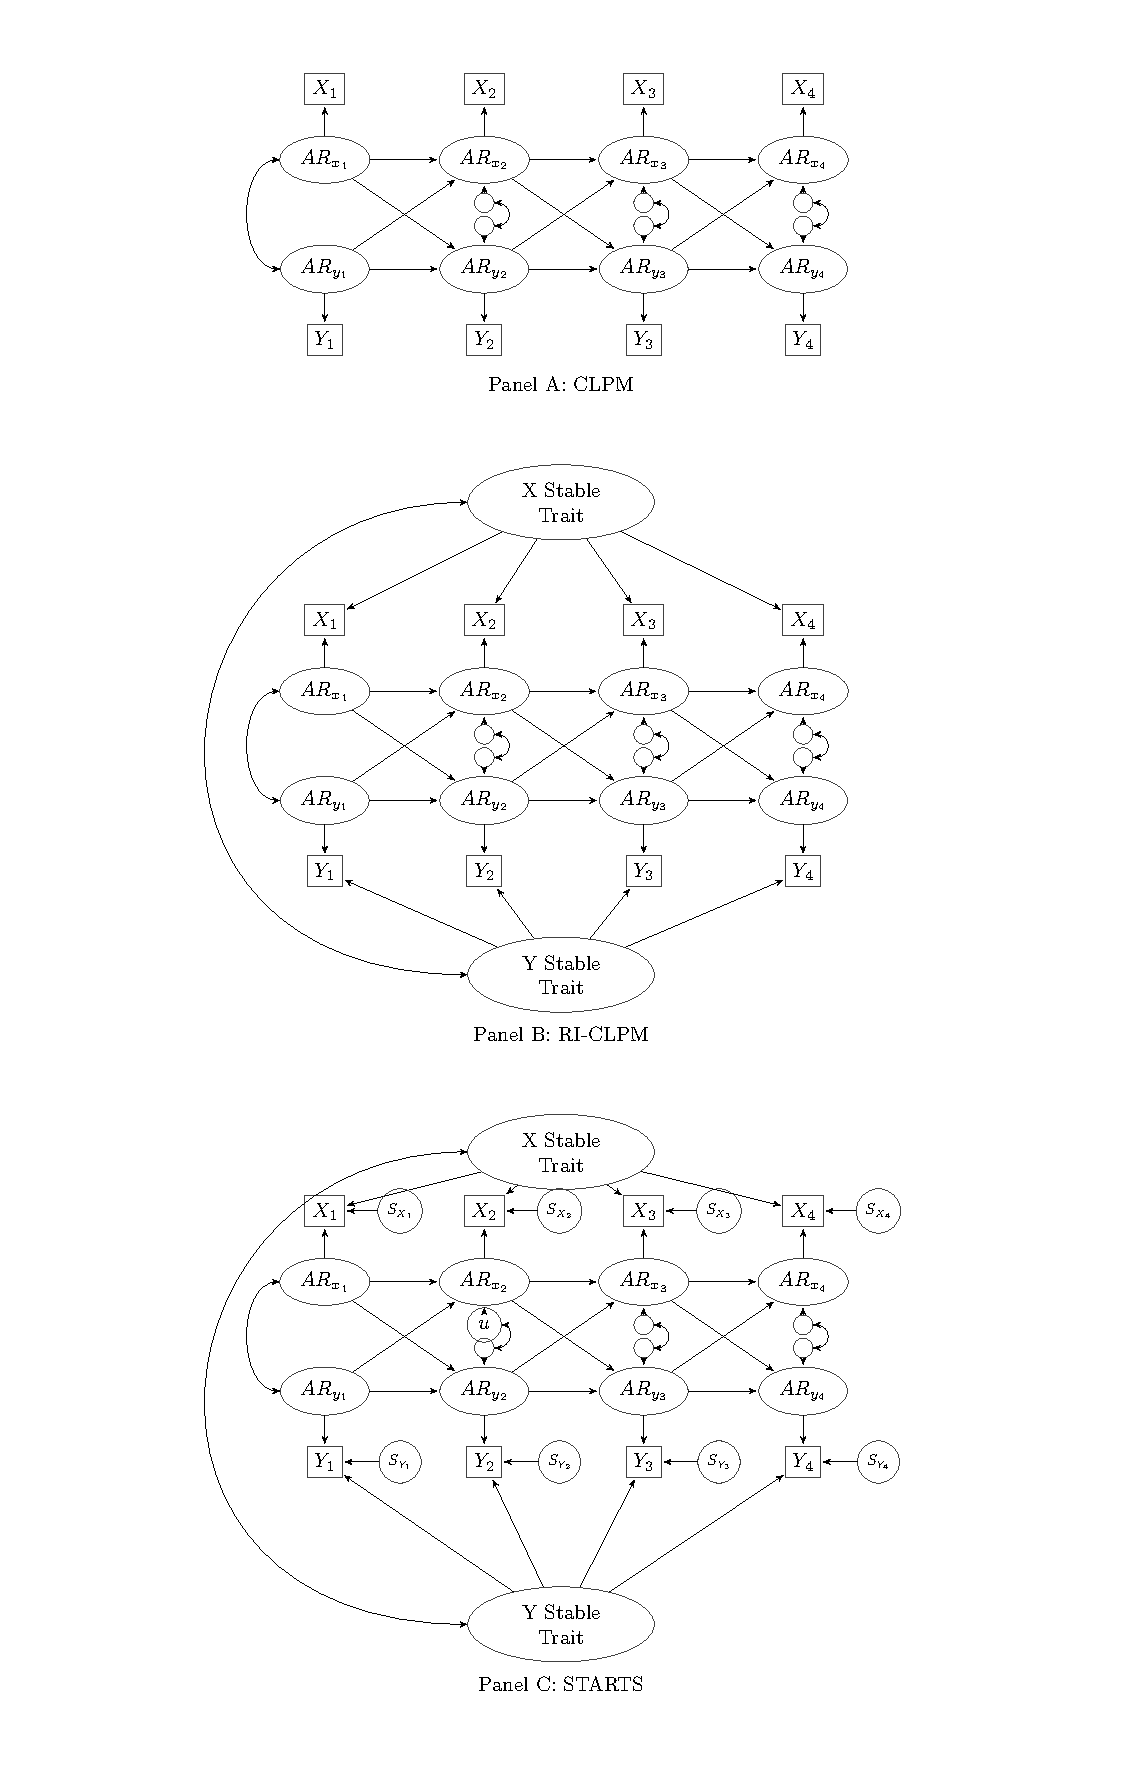
\includegraphics[height=0.9\textheight]{images/comboFigure} \caption{Diagram of the three models used in this paper.}\label{fig:riclpmFig}
\end{figure}

The difference between the CLPM and the RI-CLPM is that the RI-CLPM includes a random-intercept (labeled ``Stable Trait'' in the figure, according the STARTS terminology) that accounts for ``time-invariant, trait-like stability'' (Hamaker et al., 2015, p. 104). Including this stable-trait component changes the meaning of the autoregressive part of the model. Whereas in the CLPM, the cross-lagged paths reflect associations between the \emph{X} and \emph{Y} variables over time, in the RI-CLPM, these paths reflect associations among wave-specific deviations from a person's stable-trait level\footnote{These deviations have sometimes been described as deviations from a person's mean (e.g., Lüdtke \& Robitzsch, 2021), but this is incorrect. The random intercept in the RI-CLPM and STARTS only captures variance that is perfectly stable over time, and the autoregressive part of the model reflects deviations from this stable trait. For example, it is possible to generate data with a purely autoregressive structure and no stable trait. In these data, there might be substantial person-mean variance, but no stable-trait variance.}. This is what allows for the separation of between and within-person effects (Allison, 2009; Curran \& Bauer, 2011; Hamaker et al., 2015). Note that the CLPM is nested within the RI-CLPM; the CLPM is equivalent to the RI-CLPM with the random-intercept (or stable-trait) variance constrained to 0. This also means that if one tries to fit the RI-CLPM to data with no stable-trait variance, the interpretation of the ``within-person'' or autoregressive part of the model will be identical to the interpretation of the CLPM.

Notice that neither the CLPM nor the RI-CLPM include any measurement-error variance for the indicators. For the CLPM, this means that the latent variables from the autoregressive part of the model are equivalent to the observed variables (which is why it is also possible to draw an equivalent CLPM model with only observed variables). For the RI-CLPM, the observed variables are determined by the random intercept and the corresponding wave-specific latent variable from the autoregressive part of the model.

As can be seen in Figure \ref{fig:riclpmFig}, the STARTS model differs from the RI-CLPM in that it does include measurement error. More precisely, the STARTS includes a wave-specific ``state'' component (labeled \emph{s\textsubscript{t}} in the figure), which reflects variance in an observed variable that is perfectly ``state-like'' and unique to that occasion. Note that this state component can include measurement error or any reliable variance that is unique to a single wave of assessment. The idea that some amount of pure state variance would exist in measures of psychological constructs is quite plausible, but simpler models like the RI-CLPM have often been preferred because the STARTS requires more waves of data than the RI-CLPM and often has estimation problems (e.g., Cole, Martin, \& Steiger, 2005; Orth et al., 2021).

Recently, Usami, Murayama, and Hamaker (2019) clarified that the CLPM, RI-CLPM, STARTS and many other longitudinal models could be thought of as variations of an overarching ``unified'' model that captures many different forms of change (also see Zyphur et al., 2020). For instance, an alternative model---the Latent Curve Model with Structured Residuals (Curran, Howard, Bainter, Lane, \& McGinley, 2014)---can be thought of as an RI-CLPM with a random slope. Because debates about the utility of the CLPM have primarily focused on debates about the inclusion of the random-intercept, I focus here only on the comparison of the CLPM to the RI-CLPM and the STARTS, as this comparison highlights these debates most clearly. It is certainly true, however, that if the other forms of change included in the unified model were part of the actual data generating model, then all the models covered in this paper would be misspecified and could lead to biased estimates.

\hypertarget{the-importance-of-separating-between-person-effects-from-within-person-effects}{%
\subsection{The Importance of Separating Between-Person Effects From Within-Person Effects}\label{the-importance-of-separating-between-person-effects-from-within-person-effects}}

Data that have been collected from multiple people across multiple occasions include information both about about how people differ from one another (between-person effects) and how each person changes over time (within-person effects). Methodologists have, for many decades, warned that failure to consider multilevel structures can lead to incorrect conclusions (see Curran \& Bauer, 2011, for a review and discussion). It would be wrong, for instance, to draw conclusions about within-person effects from between-person data or to draw conclusions about between-person differences from within-person data because the association can be completely different at these different levels. In addition---and most importantly for debates about the merits of the CLPM---when data do have a multilevel structure, but this multilevel structure is not taken into account through appropriate analytic methods, the estimates obtained from analyses of these data reflect \emph{an uninterpretable mix of between and within-person effects.} Hamaker et al. (2015) emphasized that a strength of the RI-CLPM is its ability to separate between-person effects from within-person effects when examining reciprocal effects.

Critics of the RI-CLPM focus on this distinction when explaining their concerns with the model. For instance, in their critique of the RI-CLPM, Lüdtke and Robitzsch (2021) cautioned that ``researchers should be aware that within-person effects are based on person-mean centered (i.e., ipsatized) scores that only capture temporary fluctuations around individual person means'' which would be ``less appropriate for understanding the potential effects of causes that explain differences between persons'' (p.~18). The latter part of this sentence is certainly correct (though the first part is technically not\footnote{Although the isolation of within-person effects in a multilevel-modeling context is frequently accomplished through ipsatization---or deviating observed scroes from a person's mean---that is not always true in a structural equation modeling context (Curran, Lee, Howard, Lane, \& MacCallum, 2012). The within-person part of the RI-CLPM reflects deviations from the stable trait, not deviations from the person mean. These are conceptually and empirically different.}); it simply restates what methodologists who focus on multilevel data have always emphasized: Researchers cannot draw conclusions about between-person effects from within-person data. There are certainly processes that are of interest to researchers that simply do not manifest in the within-person changes that people experience and report in a typical longitudinal study. In such cases, the RI-CLPM and STARTS will not be useful, though neither will the CLPM.

Orth et al. (2021) make a similar argument, but they use it to defend the CLPM. They argue that ``a potential disadvantage of the proposed alternatives to the CLPM is that they estimate within-person prospective effects only, but not between-person prospective effects'' (p.~1014). Notably, when highlighting this issue, Orth et al. (2021) do not explain how to estimate a ``between-person prospective effect'' while also addressing the inherent difficulties that emerge when analyzing data with a multilevel structure. Remember, methodologists have shown that when data have a multilevel structure and the analyses do not account for this structure, the resulting estimates reflect an uninterpretable mix of between and within-person effects. More precisely, the estimates could reflect a purely within-person process, a purely between-person process, or some combination of the two.

The CLPM is a classic example of an analysis that fails to separate between-person effects from within. Rather than clarifying how the CLPM solves the uncontroversial interpretational issues that are inevitably involved with this type of analysis, Orth et al. (2021) completely ignore and sidestep this perennial analytic issue. If these authors believe that the CLPM somehow avoids the interpretational challenges inherent in all analyses of multilevel data, then they must do more than simply assert this to be true. Orth et al. (2021) go on to note that ``in many fields researchers are also interested in gaining information about the consequences of between-person differences'' (p.~1014). Again, this is certainly true; there are times when the within-person effects that are the focus of the RI-CLPM are not the effects of interest. But this fact does not mean that ignoring the multilevel structure of data when estimating the CLPM solves the problem.

Orth et al. (2021) defend the CLPM by providing a very literal description of what the model estimates. For instance, they state that when examining the reciprocal effects of self-esteem on depression in a traditional CLPM, significant cross-lagged paths from self-esteem to depression can be interpreted to mean that ``When individuals have low self-esteem (relative to others), they will experience a subsequent rank-order increase in depression compared to individuals with high self-esteem.'' While technically correct, this ``rank-order change'' may have nothing to do with the ``between-person prospective effect'' that Orth et al. (2021) hope to assess. Indeed, significant cross-lagged paths in the CLPM can result from purely between-person differences, purely within-person effects, or some combination of the two (even combinations where the within and between-person associations are in the opposite direction). Estimates from the CLPM are uninterpretable for all the same reasons that any analysis of multilevel data that fails to account for the multilevel structure are.

To demonstrate, I generated two waves of data for two variables \emph{X} and \emph{Y} for 10,000 people. Panel A of Figure \ref{fig:spurious} shows the data-generating model, which is a very simple correlated-latent-trait model. I set the variance of \emph{X} and \emph{Y} to be 1, and the reliability of the indicators to be .5. \emph{X} and \emph{Y} are only associated at the between-person level (\(r = .7\)). Panel B shows what happens if we fit the CLPM to these data. As can be seen in this panel, there would be strong evidence for reciprocal associations between the two, even though there are no over-time associations whatsoever. The CLPM simply cannot distinguish between associations that occur at the stable-trait level from those that incorporate some change over time.

\begin{figure}
\centering
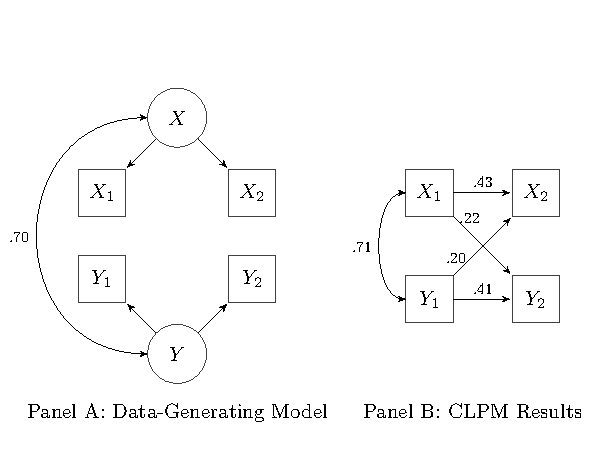
\includegraphics{images/clpm.pdf}
\caption{\label{fig:spurious}Spurious cross-lagged effects in data with only between-person associations. Panel A is the data-generating model; Panel B shows estimates from the CLPM fit to the generated data. Coefficients are unstandardized estimates.}
\end{figure}

It can sometimes be difficult to think about how the complex nature of multilevel data can affect conclusions about underlying processes. Figure \ref{fig:spurious} helps, however, by providing an alternative way of thinking about the problems with the CLPM and the benefits of alternative models that incorporate a stable-trait component. Models like the RI-CLPM and STARTS are useful because they test an extremely plausible alternative explanation of the underlying pattern of correlations that is being modeled when the CLPM is used, an alternative explanation that has nothing to do with temporal effects.

The logic of the CLPM is very similar to the logic of any other regression model where we assess whether one variable predicts another after controlling for relevant confounds. When we test whether Time 1 \emph{X} predicts Time 2 \emph{Y} after controlling for Time 1 \emph{Y}, we hope to capture whether there is something unique about \emph{X}---something that cannot be explained by the concurrent association between \emph{X} and \emph{Y}---that helps us predict \emph{Y} at a later time. But as Westfall and Yarkoni (2016) pointed out when discussing the difficulty of establishing incremental predictive validity of any kind, if the measure that we include as a control (i.e., Time 1 \emph{Y}) is not a perfect measure of what we're trying to account for, then it is possible---indeed, quite easy---to find spurious ``incremental validity'' effects. Referring to Figure \ref{fig:spurious}, \emph{Y\textsubscript{1}} is an imperfect measure of the latent variable \emph{Y}. Thus, controlling for \emph{Y\textsubscript{1}} does not control for all of the association between \emph{X} and \emph{Y}, which means that \emph{X\textsubscript{1}} will still have incremental predictive validity of \emph{Y\textsubscript{2}} even after controlling for \emph{Y\textsubscript{1}}.

In summary, decades of methodological work shows the importance of distinguishing between-person effects from within-person effects when data have a multilevel structure. Failing to do so results in uninterpretable estimates of the association between predictors and outcomes. The CLPM is not an exception to this widely discussed rule. In defending the CLPM, Orth et al. (2021) sidestep the issue of how a model that fails to distinguish between levels can lead to interpretable results; instead, they simply assert that these effects are meaningful. It is easy to show, however, that when the CLPM is used, it is possible to mistake purely between-person effects for over-time associations, which confirms the long-standing methodological warning about the failure to separate effects at different levels. I now turn to a set of simulations that demonstrate just how bad this problem likely is.

\hypertarget{its-extremely-easy-to-find-spurious-cross-lagged-effects}{%
\section{It's Extremely Easy to Find Spurious Cross-Lagged Effects}\label{its-extremely-easy-to-find-spurious-cross-lagged-effects}}

The issues discussed in the previous section show that it is possible to mistake purely between-person associations for over-time effects when the CLPM is used. But how likely are such spurious effect? Unfortunately, it is extremely easy to find spurious cross-lagged associations under conditions that are quite likely in the typical situations where the CLPM is used. Hamaker et al.~(2015) conducted simulations to show that the estimates from a cross-lagged panel model were often biased in realistic situations. I don't think they went far enough, though, in describing the practical implications of these simulations or showing just how likely spurious effects are in realistic situations. So the rest of this paper builds on their simulations and tries to clarify when such spurious effects are likely to occur. As I show, there are many realistic scenarios where researchers are almost guaranteed to find spurious cross-lagged effects.

\hypertarget{the-simulations}{%
\subsection{The Simulations}\label{the-simulations}}

When considering what types of situations to simulate, I focus on realistic scenarios for the types of data to which the CLPM is likely to be applied. For instance, it is likely that most variables that psychologists choose to study over time have a longitudinal structure where stability declines with increasing interval length (reflecting an autoregressive structure), yet this decline approaches or reaches an asymptote where further increases in interval length are no longer associated with declines in stability (reflecting the influence of a stable trait). It is also likely that most measures of psychological constructs have some amount of pure state variability, which could reflect measurement error or true state-like influences. Starting with this assumption, it is then possible to test how variation in these factors affect the estimated cross-lagged paths when the CLPM is used. A Shiny app is available where variations of this data-generating model can be specified and the effects on cross-lagged paths can be tested: \href{https://rlucas11.shinyapps.io/clpm}{rlucas11.shinyapps.io/clpm}\footnote{The app is currently deployed on shinyapps.io, but with limited monthly access time. If the site has exceeded capacity, it is also available here: \url{https://github.com/rlucas11/starts/tree/main/shiny}. Download the ``app.R'' file and the ``scripts'' folder and then run it like any other Shiny app.}. Readers can use this app to examine the specifications described in the text and to test alternatives.

Because the focus of this paper is on examining the effects of unmodeled stable trait variance, I set the variance of the stable trait component for the predictor and outcome to be 1 in the primary simulations (though occasionally, I do set stable-trait variance to zero to address specific questions). I then varied the ratio of autoregressive variance to stable-trait variance across four levels: 0, .5, 1, and 2. Similarly, I varied the ``reliability'' of the measures (defining reliability as the proportion of variance due to stable-trait and autoregressive-trait variance) across three levels: .5, .7, and .9. Even the lowest level is not unrealistic, given that the state component includes both measurement error and reliable state variance. Finally, I varied the size of the correlation between the stable traits across four levels from very weak to very strong: .1, .3, .5, and .7. I ran 1,000 simulations for each of five sample sizes: 50, 100, 250, 500, and 1,000). In all simulations, I set the correlation between the initial autoregressive variance components for the predictor and outcome to be .50 and the stability of the autoregressive components to be .50 (though, later, I discuss some modifications to this). I also set the correlations between state components to be 0. Consistent with the canonical STARTS model, I included a stationarity constraint, so that variances, correlations, and stability coefficients are constrained to be equal over time. This simplifies discussion of the estimated cross-lagged paths, as there is just one estimate per model.

After generating the data, I tested a simple two-wave CLPM, keeping track of the average size of the estimated cross-lagged paths and the number of cross-lagged paths that were significant at a level of .05. Note that researchers are often interested in determining which of the two variables in the model has a causal impact on the other rather than on simply testing the effect of one predictor on an outcome. Thus, an effect of X on Y, Y on X, or both would often be interpreted as a ``hit'' in common applications of the CLPM. This means that error rates are typically elevated in the CLPM even without unmodeled stable-trait effects unless corrections for multiple comparisons are used. In these simulations, I report the percentage of runs that result in at least one significant cross-lagged effect (out of two tested), and these can be compared to a baseline error rate of 10\%, assuming multiple comparisons are ignored.

Finally, although I focus on the common two-wave CLPM design, it is important to note that more waves of data lead to increased power to detect smaller effects---even spurious effects. This means that spurious cross-lagged associations are more likely to be found with better, multi-wave designs. Thus, I will also present results from simulations with more waves of data after presenting the primary results.

The proportion of simulations that resulted in at least one significant cross-lagged effect in this initial simulation are presented in Figure \ref{fig:simFig}. The X-axis shows results for different sample sizes. The Y-axis reflects the percentage of runs in which a significant (spurious) cross-lagged path was found. The columns reflect variation in the reliability of the measures. The rows reflect variation in the ratio of autoregressive variance to stable-trait variance. The individual lines in each plot reflect different correlations between the two stable traits. The averaged estimates for the cross-lagged paths in each set of simulations (averaging across sample sizes, as this will not affect the estimated effect) is reported in Table \ref{tab:simTab}. What do these simulations tell us about when spurious effects are likely?

\begin{figure}
\centering
\includegraphics{clpmPaper_files/figure-latex/simFig-1.pdf}
\caption{\label{fig:simFig}Simulation results for two-wave CLPM. Columns reflect different reliabilities. Rows reflect different ratios of autoregressive to stable-trait variance. Lines reflect different correlations between stable-trait components. Grey line reflects expected number of significant effects due to chance (assuming a critical p-value of .05).}
\end{figure}

\hypertarget{when-constructs-have-some-stable-trait-structure}{%
\subsubsection{When Constructs Have Some Stable-Trait Structure}\label{when-constructs-have-some-stable-trait-structure}}

If the measures include some amount of stable-trait variance--even if the stable traits are uncorrelated---it is likely that spurious cross-lagged paths will emerge. To be clear, this is most problematic when the stable traits are correlated and the correlation is quite high. However, error rates are elevated across most simulations. For instance, consider results in the third column of Figure \ref{fig:simFig}, where the reliability is a very high .9. Specifically, focus on the fourth row, where the ratio of autoregressive variance to stable-trait variance is 2:1. This panel reflects the least problematic set of values tested, and even here, error rates approach 100\% when correlations between the stable traits are strong (\emph{r} = .70) and sample sizes are large (\emph{N} = 1,000). Even when correlations are more moderate (e.g., \emph{r} = .5), however, these error rates approach 50\% in large samples.

\begin{table}[tbp]

\begin{center}
\begin{threeparttable}

\caption{\label{tab:simTab}Average Estimated Cross-Lagged Paths In Each Simulation Condition}

\begin{tabular}{rrrrr}
\toprule
 &  & \multicolumn{3}{c}{Reliability} \\
\cmidrule(r){3-5}
Stable Trait r & \multicolumn{1}{c}{AR Variance Ratio} & \multicolumn{1}{c}{0.5} & \multicolumn{1}{c}{0.7} & \multicolumn{1}{c}{0.9}\\
\midrule
0.10 & 0\% & 0.03 & 0.02 & 0.01\\
 & 50\% & 0.03 & 0.01 & -0.02\\
 & 100\% & 0.03 & 0.01 & -0.03\\
 & 200\% & 0.04 & 0.02 & -0.02\\ \midrule
0.30 & 0\% & 0.08 & 0.06 & 0.03\\
 & 50\% & 0.07 & 0.05 & 0.01\\
 & 100\% & 0.07 & 0.05 & 0.01\\
 & 200\% & 0.07 & 0.05 & 0.01\\ \midrule
0.50 & 0\% & 0.13 & 0.12 & 0.06\\
 & 50\% & 0.11 & 0.10 & 0.05\\
 & 100\% & 0.10 & 0.09 & 0.04\\
 & 200\% & 0.09 & 0.08 & 0.04\\ \midrule
0.70 & 0\% & 0.20 & 0.20 & 0.11\\
 & 50\% & 0.16 & 0.16 & 0.10\\
 & 100\% & 0.14 & 0.14 & 0.09\\
 & 200\% & 0.12 & 0.11 & 0.07\\
\bottomrule
\end{tabular}

\end{threeparttable}
\end{center}

\end{table}

Interestingly, error rates are not always monotonically associated with the size of the correlation when reliability is high. Consider the panels in Rows 2, 3, and 4 of Column 3. In these panels, where the ratio of autoregressive variance to stable-trait variance is .5 or higher, the error rates for the lowest correlation tested (\emph{r} = .1, shown in the solid line) are actually higher than error rates for a higher stable-trait correlation of .3. A look at the actual estimates across simulations in Table \ref{tab:simTab} provides insight into why this is. This table shows that the average estimated cross-lagged path is actually negative when reliability is high, the correlation between the stable traits is low, and there is substantial amounts of autoregressive variance. These negative estimates emerge even though all associations among the latent components were specified to be positive.

This effect can be demonstrated even more clearly by simulating data with uncorrelated stable traits, an equal amount of autoregressive and stable-trait variance, and no state variance whatsoever (this simulation is not shown in the figure). In this case, the estimated cross-lagged paths will be approximately -.07. This is due to the fact that by failing to account for the stable trait, the model overestimates the stability of \emph{X} and \emph{Y}, which means that the observed correlation between \emph{X} at Time 1 and \emph{Y} at Time 2 is lower than what would be expected based on the initial correlation between \emph{X} and \emph{Y} at Time 1 and the stability over time\footnote{This can be understood by using tracing rules. If we randomly generate data for 10,000 participants from the data-generating model just described, the correlation between \emph{X\textsubscript{1}} and \emph{X\textsubscript{2}} and between \emph{Y\textsubscript{1}} and \emph{Y\textsubscript{2}} are both around .75. The correlation between \emph{X\textsubscript{1}} and \emph{Y\textsubscript{1}} would be about .25, and the correlation between \emph{X\textsubscript{1}} and \emph{Y\textsubscript{2}} would be about .12. Fitting a CLPM to these data results in estimated stabilities for \emph{X} and \emph{Y} of approximately .77, and a correlation between \emph{X\textsubscript{1}} and \emph{Y\textsubscript{1}} of .25. These values would imply an observed correlation of \(.77 * .25 = .19\) between \emph{X\textsubscript{1}} and \emph{Y\textsubscript{2}}, which is greater than the actual correlation of .12. This discrepancy between the predicted and observed correlations results in the negative estimates for the cross-lagged paths.}. These simulations show that when the variables being examined have a trait-like structure, this can lead to spurious cross-lagged effects, even when the stable trait variance is not correlated. When correlations at the stable-trait level are strong, however, the effects of ignoring the stable-trait structure can be substantial. In some realistic scenarios (e.g., moderate correlations between stable traits, reliabilities of .70, and sample sizes over 100), significant spurious correlations are almost guaranteed.

\hypertarget{when-measures-have-error-or-reliable-occasion-specific-variance}{%
\subsubsection{When Measures Have Error or Reliable Occasion-Specific Variance}\label{when-measures-have-error-or-reliable-occasion-specific-variance}}

The simulations described above focus on situations where reliability is very high. When there is measurement error or reliable state variance (as is very likely), this effect gets worse---potentially \emph{much} worse. Consider the panel in the first row and the first column of Figure \ref{fig:simFig}. In this case, reliability is set to .5 and there is no autoregressive variance. Error rates are very high, approaching 100\% with large samples, even when the stable-trait correlation is just .3. Samples of 100 can result in spurious cross-lagged effects approximately 60\% of the time when stable traits are correlated .5. Even in samples as small as 50, error rates exceed 25\% in many situations.

This outcome is actually quite easy to understand. Indeed, we don't really need simulations at all to predict it. This result is a simple consequence of the issues that Westfall and Yarkoni (2016) discussed and those that I highlighted in Figure \ref{fig:spurious}. Because \emph{X} and \emph{Y} are measured with error at each occasion, controlling for Time 1 \emph{Y} when predicting Time 2 \emph{Y} from Time 1 \emph{X} does not fully account for the true association between \emph{X} and \emph{Y}. There will still be a residual association between Time 1 \emph{X} and Time 2 \emph{Y}, which can be accounted for by the freed cross-lagged path in the CLPM. The RI-CLPM (and the STARTS) are useful because they do a better job accounting for this underlying association than the CLPM.

One might argue that a model that just includes stable-trait variance and error (which is true of all simulations in the first row of Figure \ref{fig:simFig}) is unrealistic, as there is sure to be some form of autoregressive structure to most variables psychologists study. That is true, but as the other rows of the figure show, the existence of this stable trait causes problems for the CLPM even when all three sources of variability (stable trait, autoregressive trait, and state) exist.

At this point, it is important to highlight the fact that at least some of these effects are due more to the existence of measurement error (or reliable state variance) than to the existence of the stable trait. For instance, we could simulate data with an autoregressive structure, set the variance of the stable trait components to be 0, and specify no cross-lagged paths. Even with relatively high reliability (e.g., .8 for this simulation, which is not shown in the figure), the average estimated cross-lagged paths would be 0.05 and spurious effects would be found 40\% of the time in a two-wave design with samples of 500 participants. Again, Westfall and Yarkoni's (2016) explanation can account for these results: The existence of measurement error or state variance in the observed measures of \emph{Y} means that controlling for \emph{Y\textsubscript{1}} does not control for enough. The result is a spurious cross-lagged path.

It is also important to note that measurement error also affects estimates from the RI-CLPM. If we specify a data-generating model that includes all three sources of variance (stable trait, autoregressive trait, and state/measurement error), but no cross-lagged paths, the CLPM will find substantial cross-lagged effects, but so will the RI-CLPM (at least if the autoregressive components of \emph{X} and \emph{Y} are correlated). To demonstrate, I simulated data with the following characteristics. The \emph{X} and \emph{Y} stable traits had variances of 1 and a correlation of .5 and \emph{X} and \emph{Y} autoregressive traits had a variance of 1 and a starting correlation of .5 with stability coefficients of .5. The average estimated cross-lagged path was 0.07, which would be easily detectable with moderate to large sample sizes.

To examine this issue more systematically and to compare the likelihood of finding spurious effects when using the RI-CLPM to the likelihood when using the CLPM, I repeated the primary simulation using the RI-CLPM. Because the estimates of the cross-lagged paths are not affected by the size of the correlation between the stable trait components when the RI-CLPM is used, instead of varying the correlation between stable traits, I varied the correlation between the initial wave autoregressive components. In addition, the RI-CLPM requires three waves of data instead of the two that I used in the initial simulation. The results are shown in Figure \ref{fig:riSpurious}.

\begin{figure}
\centering
\includegraphics{clpmPaper_files/figure-latex/riSpurious-1.pdf}
\caption{\label{fig:riSpurious}Simulation results for three-wave RI-CLPM. Columns reflect different reliabilities. Rows reflect different ratios of autoregressive to stable-trait variance. Lines reflect different correlations between autoregressive-trait components. Grey line reflects expected number of significant effects due to chance (assuming a critical p-value of .05).}
\end{figure}

As can be seen in this figure, when there is measurement error variance or reliable state variance, then there is a chance for spurious cross-lagged paths even when the RI-CLPM is used. To be sure, these effects are much less likely than with the CLPM: Error rates typically only exceeded 25\% with large samples and very strong correlations between the autoregressive traits, whereas they often approached 100\% with the CLPM. Note, this limitation of the RI-CLPM is not an argument \emph{for} the CLPM (though it is an argument for using the STARTS or other more complicated models, when possible).

One response to the above simulations is to suggest that we simply need to use very reliable measures or perhaps model latent variables at each occasion instead of relying on observed variables with less than perfect reliability. This will certainly help, but it is important to remember that the ``state'' component in the STARTS model includes measurement error \emph{and} reliable occasion-specific variance. Reliable state variance will affect these results in exactly the same way as random measurement error. Unfortunately, we don't know how common this reliable state component is in real data, though we have at least some evidence that it can exist and be large enough to be meaningful (Lucas \& Donnellan, 2012). Thus, even the use of latent occasions in the CLPM can't solve this problem.

\hypertarget{when-there-are-many-assessment-waves}{%
\subsubsection{When There Are Many Assessment Waves}\label{when-there-are-many-assessment-waves}}

Although the CLPM is often used with just two waves of assessment, it can also be used with more complex data. Indeed, a general rule for longitudinal data is that more waves are better than fewer, and in situations where stationarity could reasonbly be expected, including more waves and imposing equality constraints should lead to more precise estimates of cross-lagged paths. When estimating true effects, this has the benefit of increasing power. When spurious effects would be expected, however, the use of more waves will also increase the probability of those spurious effects being significant (again, see Westfall \& Yarkoni, 2016, for a discussion of how factors that improve power can increase the ability to find spurious effects).

\begin{figure}
\centering
\includegraphics{clpmPaper_files/figure-latex/simFig5-1.pdf}
\caption{\label{fig:simFig5}Simulation results for five-wave CLPM. Columns reflect different reliabilities. Rows reflect different ratios of autoregressive to stable-trait variance. Lines reflect different correlations between stable-trait components. Grey line reflects expected number of significant effects due to chance (assuming a critical p-value of .05).}
\end{figure}

Figure \ref{fig:simFig5} shows a set of simulations that are similar to those reported in Figure \ref{fig:simFig}, but this time using five waves of data and the CLPM with equality constraints across waves. When comparing these two figures, the effect of increasing the number of waves is immediately apparent: Error rates increase considerably. For instance, in the very realistic scenario of an N of 250, a correlation between stable traits of .5, reliabilities of .7, and a 1:1 ratio of stable-trait to autoregressive variance, the error rate increases from 58.10\% to \% when moving from a two-wave study to a five-wave study. With five waves of data, error rates often exceed 50\%, even in samples as small as 50. So features that are generally desirable---large sample sizes and multiple waves of assessment---increase the likelihood of finding spurious cross-lagged paths.

\hypertarget{the-ri-clpm-is-not-conservative}{%
\subsection{The RI-CLPM Is Not Conservative}\label{the-ri-clpm-is-not-conservative}}

The examples above focused almost entirely on cases where there were no true cross-lagged associations in the data-generating model. The simulations showed that spurious paths are often very likely to be found. This pattern matches the intuition that the RI-CLPM is more conservative than the CLPM (Lüdtke \& Robitzsch, 2021). However, failure to model associations between stable-trait components can also lead to the \emph{underestimation} of real cross-lagged paths. For instance, consider a situation where the measures are perfectly reliable and the stable trait and autoregressive trait contribute equally (in this particular case, I also specified the correlations among the stable trait and autoregressive traits to be .5). If we simulate data with cross lagged paths of .5 from X to Y and .2 from Y to X, the RI-CLPM reproduces these effects perfectly. However, even with no measurement error, the estimates from the CLPM are half the size that they should be, approximately .25 and .10.

The precise manner in which estimates will be affected depends on the size of these variance components and the correlations between them. Table \ref{tab:truePaths} shows the results from a separate simulation that examines these effects. Specifically, because the parameter estimates were the focus (rather than the frequency of errors), I followed Lüdtke and Robitzsch (2021) and generated just one set of 10,000 responses for each of 48 combinations. I varied the correlation between the stable traits across four levels: .1, .3, .5, and .7. Similarly, I varied the correlation between the autoregressive traits across the same four levels. I also varied the ratio of autoregressive to trait variance across three levels: .5, 1, and 2. For this example, reliability was set to be 1 and the stability of the autoregressive components were set to .5. The table only shows results for one cross-lagged path, for which the true value is .50.

\begin{table}[tbp]

\begin{center}
\begin{threeparttable}

\caption{\label{tab:truePaths}Average Estimated Cross-Lagged Path In Each Simulation Condition When True Value = .5.}

\begin{tabular}{rrrrrr}
\toprule
 &  & \multicolumn{4}{c}{Stable Trait Correlation} \\
\cmidrule(r){3-6}
AR r & \multicolumn{1}{c}{AR Ratio} & \multicolumn{1}{c}{0.1} & \multicolumn{1}{c}{0.3} & \multicolumn{1}{c}{0.5} & \multicolumn{1}{c}{0.7}\\
\midrule
0.10 & 0.50 & 0.17 & 0.20 & 0.24 & 0.30\\
0.10 & 1.00 & 0.26 & 0.29 & 0.33 & 0.38\\
0.10 & 2.00 & 0.33 & 0.37 & 0.38 & 0.43\\ \midrule
0.30 & 0.50 & 0.15 & 0.16 & 0.20 & 0.26\\
0.30 & 1.00 & 0.22 & 0.25 & 0.28 & 0.35\\
0.30 & 2.00 & 0.31 & 0.32 & 0.37 & 0.42\\ \midrule
0.50 & 0.50 & 0.11 & 0.13 & 0.16 & 0.23\\
0.50 & 1.00 & 0.18 & 0.21 & 0.25 & 0.31\\
0.50 & 2.00 & 0.25 & 0.29 & 0.33 & 0.39\\ \midrule
0.70 & 0.50 & 0.07 & 0.09 & 0.12 & 0.17\\
0.70 & 1.00 & 0.12 & 0.15 & 0.19 & 0.25\\
0.70 & 2.00 & 0.20 & 0.23 & 0.28 & 0.34\\
\bottomrule
\addlinespace
\end{tabular}

\begin{tablenotes}[para]
\normalsize{\textit{Note.} AR r = Correlation between autoregressive components; AR Ratio = Ratio of autoregressive variance to stable-trait variance. Reliability is set to 1 for all simulations.}
\end{tablenotes}

\end{threeparttable}
\end{center}

\end{table}

First consider the example just discussed. Looking at the column where the correlation between the stable traits is .5, and the row where the correlation between the autoregressive traits is .5 and the ratio of autoregressive variance to stable-trait variance is 1, the true cross-lagged path of .5 is estimated to be .25. One can then move up and down that column or across that row to see the effects of the other factors on this underestimation. For instance, looking at the values in the rows immediately above and below this value shows that the underestimation of the cross-lagged paths is greater when there is more stable trait variance than when there is less. The true cross-lagged path of .50 is estimated to be .16 when there is twice as much stable trait variance as autoregressive variance, whereas it is estimated to be .33 (still an underestimate, but not as bad), when there is twice as much autoregressive variance as stable-trait variance.

Moving across the same row shows how this estimate is affected by variation in the correlation between stable traits. As can be seen, the estimate for a true cross-lagged association of .50 declines from .31 when the correlation between the stable traits is a high .70 to .25 when the correlation is .50, to .21 when the correlation is .30, to .18 when the correlation is 0.1. Again, stable trait variance affects estimates of cross-lagged paths even when the stable traits are uncorrelated.

Finally, moving across groups of rows (e.g., Rows 1 through 3 compared to Rows 4 through 6) shows the effect of the correlation between autoregressive components. In this case, the estimate of the cross-lagged parameter is \emph{negatively} associated with the size of the correlation between autoregressive components, declining from .33 when the correlation between autoregressive components is .10 to .19 when the correlation is .70 (again, for the example where the stable-trait correlation is .5 and there is an equal amount of autoregressive and stable-trait variance).

These simulations show that the RI-CLPM is not more conservative than the CLPM when testing cross-lagged effects. Indeed, when true cross-lagged associations exist, the CLPM is likely to underestimate them. Again, this pattern is actually easily predictable just by considering tracing rules for structural equation models. When stable-trait variance exists, the stability of the observed variables is overestimated in a CLPM, resulting in a corresponding underestimation of the cross-lagged paths in most situations. If researchers observe a pattern where cross-lagged paths routinely emerge when the CLPM is used but these paths disappear when the RI-CLPM is applied, then this would suggest that the effects themselves are likely spurious.

When considering the implications of this finding, there are two things to keep in mind. First, although the CLPM typically underestimates the true cross-lagged paths, this may not result in decreased power to detect effects relative to alternative models like the RI-CLPM. This is partly due to the fact that models that separate between-person effects from within frequently have less bias, but at the cost of efficiency; the standard errors in such models are often greater than models that do not correctly separate levels (see Allison, 2009, for an explanation). Second, it is difficult to consider how to think about power in the context of the CLPM, where it is so easy to find spurious effects. Indeed, I attempted to run simulations similar to those described earlier, but with true cross-lagged effects. However, when simulating data where one cross-lagged path was zero and the other was greater than zero, estimated ``power'' to detect either the true effect or the spurious one were quite high.

The second thing to remember is that the above simulations were conducted specifying that the measures are perfectly reliable and that there is no occasion-specific state variance. This is unlikely in practice. Indeed, when state variance is included, the estimates from the RI-CLPM are also biased. The precise way that state variance impacts estimates is a quite complicated function of all the factors included in the previous simulations, the state factor, and the direction of the correlations and true cross-lagged paths. Because of this complexity, these simulations are beyond the scope of this paper, though the Shiny app is provided for readers to examine the effect of different combinations on estimated cross-lagged paths. Importantly, the STARTS model is appropriate for modeling data that includes stable-trait, autoregressive-trait, and state variance. Although the STARTS model has been somewhat underused in the literature because of frequent estimation problems, recent methodological advances in Bayesian modeling have helped address these concerns (Lüdtke, Robitzsch, \& Wagner, 2018).

\hypertarget{moving-forward-with-the-clpm}{%
\subsection{Moving Forward with the CLPM}\label{moving-forward-with-the-clpm}}

After describing the various approaches available to model longitudinal data, Orth et al. (2021) made the following recommendation: ``Before selecting a model, researchers should carefully consider the psychological or developmental process they would like to examine in their research, and then select a model that best estimates that process.'' This sounds like advice with which no one could argue. But if there is a plausible alternative model that describes the data as well as (or better than) the preferred model, then much more work is needed to defend that selection.

As an obvious example, if the true causal process linking self-esteem to depression is that changes in self-esteem instantaneously cause a corresponding change in depression (and there are no confounding factors), then that causal effect would be perfectly captured by the cross-sectional correlation between the two variables. Indeed, it would actually be problematic to rely on the cross-lagged association between self-esteem and depression controlling for earlier levels of depression as an estimate of the causal effect. Yet few would find a cross-sectional correlation between self-esteem and depression to be compelling evidence for a causal effect of self-esteem even if a researcher's preferred process only predicted such cross-sectional associations. This is because there are so many plausible alternative models that explain that cross-sectional effect. Unfortunately, the situation is no better with longitudinal data tested using the CLPM.

When researchers acquire data from multiple people on multiple occasions, that data has a multilevel structure; this point is uncontroversial. It is also uncontroversial to note that when multilevel data are analyzed using analytic approaches that do not separate these levels, the estimates from those models reflect an uninterpretable mix of between and within-person effects. Perhaps there is some reason why this long-standing and well-documented concern about the analysis of multilevel data does not apply in the case of the CLPM, but Orth et al. (2021) did not articulate such a reason. Indeed, they did not acknowledge this problem or discuss how the CLPM solves it. Moreover, it is quite easy to show that the CLPM simply cannot distinguish between the ``between-person prospective effects'' Orth et al. (2021) claim to want to test and simple between-person differences.

It is noteworthy that Orth et al. (2021) did not propose a data-generating model that would result in biased estimates or incorrect conclusions if modeled using the RI-CLPM. It is easy to show that generating data from the model that they claim to prefer---the CLPM---results in correct estimates (despite inadmissable solutions due to negative estimated variances) when analyzed using the RI-CLPM. I believe that it is not possible to specify a data-generating model that corresponds to the processes that the critics describe that would also lead to incorrect estimates when analyzed using the RI-CLPM\footnote{Lüdtke and Robitzsch (2021) did show that the RI-CLPM cannot successfully control for all types of confounds, but this is an issue that is distinct from the question of whether we can simply recover the structure of these variables over time. Of course, it is possible to specify data-generating models that do result in data that, when analyzed using the RI-CLPM, lead to incorrect conclusions (including the more complex models described by Usami et al. (2019)). My point is that the critics of the RI-CLPM have not provided a model that matches the processes that they describe and also results in incorrect estimates when modeled using the RI-CLPM.}.

In addition to these conceptual reasons for abandoning the CLPM, the simulations reported in this paper show that relying on the CLPM when the variables in the model have some stable trait variance leads to dramatically inflated error rates (often reaching 100\% in realistic scenarios, even with small to moderate sample sizes). The constructs that psychologists study very rarely have a purely autoregressive structure. At some point, the long-term stabilities of most constructs are stronger than would be suggested by the short-term stabilities and the length of time that has elapsed alone. This is likely due to the fact that many constructs have at least some stable-trait variance that is maintained over time. And if there is stable trait variance, it is quite plausible that two constructs correlate at the stable-trait level. The RI-CLPM and STARTS models provide a way to test this compelling and plausible model and to adjust for the problematic effects of these stable-trait components for the estimation of reciprocal effects.

So, if using the CLPM results in dramatically elevated error rates for cross-lagged paths when they do not exist, while also underestimating estimates of these associations when they do exist (again, sometimes dramatically in realistic scenarios), should we ever rely on the CLPM for causal analyses? My suggestion in the title of this paper that the CLPM be abandoned was not intended to be attention-grabbing hyperbole; it simply reflects the difficulty identifying any situation where the CLPM would be preferable to alternatives. When at least three waves of data are available, the RI-CLPM can be used. If no stable trait variance exists, the RI-CLPM will simply reduce to a CLPM.

To be sure, there are certain situations when alternatives to the CLPM cannot be used, most notably in the very common situation where only two waves of assessment are available. However, as Figure \ref{fig:spurious} showed, there are too many plausible alternative models that can lead to the same set of six correlations among two variables at two time points to draw any conclusions about which of those models is correct. Many have suggested that two-wave designs barely count as ``longitudinal'' (e.g., Ployhart \& MacKenzie, 2014; Rogosa, 1995), and their reasons for this claim are quite salient when considering the application of the CLPM to such data. There is simply not enough information available in these data to distinguish among multiple competing models. In discussing reciprocal associations using cross-lagged analyses, Rogosa (1995) noted that there is a ``hierarchy of research questions about longitudinal data {[}that{]} might start with describing how a single attribute---say aggression---changes over time. A next step would be questions about individual differences in change of aggression over time, especially correlates of change in aggression. Only after such questions are well understood does it seem reasonable to address a question about feedback or reciprocal effects, such as how change in aggression relates to change in exposure to TV violence or, does TV violence cause aggressive behavior?'' (p.~34). Many researchers have noted that this first step---describing how a construct changes over time---is not possible with only two waves of data (e.g., Fraley \& Roberts, 2005; Ployhart \& MacKenzie, 2014; Rogosa, 1995). Because we cannot understand the longitudinal structure of the variables with two waves of data, the estimates from a two-wave CLPM are uninterpretable.

All researchers want to obtain information about the phenomena they study as efficiently as possible. The widely used CLPM is a simple analysis that can be applied in many situation with very little data. Unfortunately, this simple model is not up to the task of clarifying causal processes in longitudinal data. By failing to separate between-person and within-person levels, the CLPM cannot distinguish over-time effects from simple between-person associations. Simulation studies show that the CLPM results in extremely elevated error rates when stable-trait (or state) variance exists; spurious associations are very likely in many different realistic scenarios. This confirms what methodologists have highlighted for many years: By failing to account for the multilevel structure of longitudinal data, models like the CLPM result in uninterpretable estimates. Berry and Willoughby (2017) suggested that it was time to ``rethink'' the CLPM, which they described as a workhorse of developmental research. The introduction of useful alternatives like the RI-CLPM and STARTS, when combined with the simulations from this show that it is time for this workhorse to be retired.

\hypertarget{references}{%
\section*{References}\label{references}}
\addcontentsline{toc}{section}{References}

\hypertarget{refs}{}
\begin{CSLReferences}{1}{0}
\leavevmode\vadjust pre{\hypertarget{ref-allison2009fixed}{}}%
Allison, P. D. (2009). \emph{Fixed effects regression models}. {Sage}.

\leavevmode\vadjust pre{\hypertarget{ref-berry_practical_2017}{}}%
Berry, D., \& Willoughby, M. T. (2017). On the {Practical Interpretability} of {Cross-Lagged Panel~Models}: {Rethinking} a {Developmental Workhorse}. \emph{Child Development}, \emph{88}(4), 1186--1206. \url{https://doi.org/gbf8jt}

\leavevmode\vadjust pre{\hypertarget{ref-cole_empirical_2005}{}}%
Cole, D. A., Martin, N. C., \& Steiger, J. H. (2005). Empirical and {Conceptual Problems With Longitudinal Trait-State Models}: {Introducing} a {Trait-State-Occasion Model}. \emph{Psychological Methods}, \emph{10}(1), 3--20. \url{https://doi.org/10.1037/1082-989x.10.1.3}

\leavevmode\vadjust pre{\hypertarget{ref-curran_disaggregation_2011}{}}%
Curran, P. J., \& Bauer, D. J. (2011). The {Disaggregation} of {Within-Person} and {Between-Person Effects} in {Longitudinal Models} of {Change}. \emph{Annual Review of Psychology}, \emph{62}(1), 583--619. \url{https://doi.org/d54m6f}

\leavevmode\vadjust pre{\hypertarget{ref-curran_separation_2014}{}}%
Curran, P. J., Howard, A. L., Bainter, S. A., Lane, S. T., \& McGinley, J. S. (2014). The separation of between-person and within-person components of individual change over time: {A} latent curve model with structured residuals. \emph{Journal of Consulting and Clinical Psychology}, \emph{82}(5), 879--894. \url{https://doi.org/10.1037/a0035297}

\leavevmode\vadjust pre{\hypertarget{ref-curran_disaggregating_2012}{}}%
Curran, P. J., Lee, T., Howard, A. L., Lane, S., \& MacCallum, R. (2012). Disaggregating {Within-Person} and {Between-Person Effects} in {Multilevel} and {Structural Equation Growth Models}. In \emph{Advances in {Longitudinal Methods} in the {Social} and {Behavioral Sciences}} (pp. 217--253). {Information Age Publishing}.

\leavevmode\vadjust pre{\hypertarget{ref-Fraley2005PR}{}}%
Fraley, R. C., \& Roberts, B. W. (2005). Patterns of {Continuity}: {A Dynamic Model} for {Conceptualizing} the {Stability} of {Individual Differences} in {Psychological Constructs Across} the {Life Course}. \emph{Psychological Review}, \emph{112}(1), 60--74. \url{https://doi.org/10.1037/0033-295X.112.1.60}

\leavevmode\vadjust pre{\hypertarget{ref-hamaker_critique_2015}{}}%
Hamaker, E. L., Kuiper, R. M., \& Grasman, R. P. P. P. (2015). A critique of the cross-lagged panel model. \emph{Psychological Methods}, \emph{20}(1), 102--116. \url{https://doi.org/f67cvh}

\leavevmode\vadjust pre{\hypertarget{ref-kenny_trait_1995}{}}%
Kenny, D. A., \& Zautra, A. (1995). The trait-state-error model for multiwave data. \emph{Journal of Consulting and Clinical Psychology}, \emph{63}(1), 52--59. \url{https://doi.org/10.1037/0022-006X.63.1.52}

\leavevmode\vadjust pre{\hypertarget{ref-Kenny2001}{}}%
Kenny, D. A., \& Zautra, A. (2001). The trait-state models for longitudinal data. In L. M. Collins \& A. G. Sayer (Eds.), \emph{New {Methods} for the {Analysis} of {Change}} (pp. 243--263). {Washington, DC}: {American Psychological Association}.

\leavevmode\vadjust pre{\hypertarget{ref-LucasInPressSIR}{}}%
Lucas, R. E., \& Donnellan, M. B. (2012). Estimating the {Reliability} of {Single-Item Life Satisfaction Measures}: {Results} from {Four National Panel Studies}. \emph{Social Indicators Research}, \emph{3}, 323--331.

\leavevmode\vadjust pre{\hypertarget{ref-ludtke_critique_2021}{}}%
Lüdtke, O., \& Robitzsch, A. (2021). A {Critique} of the {Random Intercept Cross-Lagged Panel Model}. {PsyArXiv}. \url{https://doi.org/10.31234/osf.io/6f85c}

\leavevmode\vadjust pre{\hypertarget{ref-ludtke_more_2018}{}}%
Lüdtke, O., Robitzsch, A., \& Wagner, J. (2018). More stable estimation of the {STARTS} model: {A Bayesian} approach using {Markov} chain {Monte Carlo} techniques. \emph{Psychological Methods}, \emph{23}(3), 570--593. \url{https://doi.org/gd86g5}

\leavevmode\vadjust pre{\hypertarget{ref-orth_testing_2021}{}}%
Orth, U., Clark, D. A., Donnellan, M. B., \& Robins, R. W. (2021). Testing prospective effects in longitudinal research: {Comparing} seven competing cross-lagged models. \emph{Journal of Personality and Social Psychology}, \emph{120}(4), 1013--1034. \url{https://doi.org/gg7zfw}

\leavevmode\vadjust pre{\hypertarget{ref-ployhart_two_2014}{}}%
Ployhart, R. E., \& MacKenzie, W. I. (2014). Two {Waves} of {Measurement Do Not} a {Longitudinal Study Make}. In C. E. Lance \& R. J. Vandenberg (Eds.), \emph{More {Statistical} and {Methodological Myths} and {Urban Legends}} (pp. 85--99). {Routledge}.

\leavevmode\vadjust pre{\hypertarget{ref-rogosa_myths_1995}{}}%
Rogosa, D. R. (1995). Myths and methods: "{Myths} about longitudinal research" plus supplemental questions. In J. M. Gottman (Ed.), \emph{The {Analysis} of {Change}} (pp. 3--66). {Mahwah, NJ}: {Lawrence Erlbaum Associates}.

\leavevmode\vadjust pre{\hypertarget{ref-usami_differences_2020}{}}%
Usami, S. (2020). On the {Differences} between {General Cross-Lagged Panel Model} and {Random-Intercept Cross-Lagged Panel Model}: {Interpretation} of {Cross-Lagged Parameters} and {Model Choice}. \emph{Structural Equation Modeling: A Multidisciplinary Journal}, \emph{0}(0), 1--14. \url{https://doi.org/gj6znt}

\leavevmode\vadjust pre{\hypertarget{ref-usami_unified_2019}{}}%
Usami, S., Murayama, K., \& Hamaker, E. L. (2019). A unified framework of longitudinal models to examine reciprocal relations. \emph{Psychological Methods}, \emph{24}(5), 637--657. \url{https://doi.org/gf4fqx}

\leavevmode\vadjust pre{\hypertarget{ref-westfall_statistically_2016}{}}%
Westfall, J., \& Yarkoni, T. (2016). Statistically {Controlling} for {Confounding Constructs Is Harder} than {You Think}. \emph{PLOS ONE}, \emph{11}(3), e0152719. \url{https://doi.org/10.1371/journal.pone.0152719}

\leavevmode\vadjust pre{\hypertarget{ref-zyphur_data_2020}{}}%
Zyphur, M. J., Allison, P. D., Tay, L., Voelkle, M. C., Preacher, K. J., Zhang, Z., \ldots{} Diener, E. (2020). From {Data} to {Causes I}: {Building A General Cross-Lagged Panel Model} ({GCLM}). \emph{Organizational Research Methods}, \emph{23}(4), 651--687. \url{https://doi.org/gf8rt5}

\end{CSLReferences}


\end{document}
